\documentclass[11pt,a4paper]{article}

\usepackage[brazil]{babel}
\usepackage[utf8]{inputenc}
\usepackage[T1]{fontenc}
\usepackage{graphicx}
\usepackage{float}
\usepackage{amsmath}
\floatstyle{boxed}
\restylefloat{figure}
\author{Carlos Eduardo Elmadjian, Ricardo Mikio Morita e Gil Santaella}
\author{
  Elmadjian, Carlos Eduardo\\
  \texttt{elmadjian@linux.ime.usp.br}
  \and
  Morita, Ricardo Mikio\\
  \texttt{ricardom@linux.ime.usp.br}
  \and
  Santaella, Gil\\
  \texttt{gssantaella@gmail.com}
}
\linespread{1}

\title{Manual do Desenvolvedor: Canoagem}
\begin{document}
\maketitle

\section*{Introdução}
\thispagestyle{empty}
\begin{center}
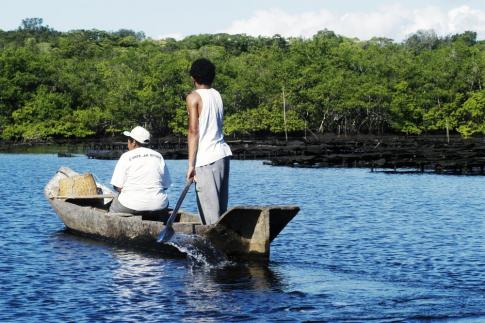
\includegraphics[scale=0.75]{canoa.jpg}
\end{center}
\begin{flushright}
{\footnotesize \textit{"Nessa canoa furada\\ remando contra a maré \\ Não acredito em nada \\ até duvido da fé"}\\ \textbf{Rita Lee}}
\end{flushright}

Este documento tem como papel descrever o funcionamento do executável de Canoagem para o desenvolvedor. Nas seções a seguir, descreveremos o funcionamento do programa.

\section{Compilação}
\setcounter{page}{1}
	O programa principal está contido em \verb|main.c|, o qual depende dos seguintes outros 	arquivos-fontes: \\

\begin{itemize}
\item \textbf{config.h} $\rightarrow$ Interface de config.c
\item \textbf{config.c} $\rightarrow$ Contém rotinas de tratamento de entrada, de abertura de arquivos e de configuração do programa
\item \textbf{debugger.h} $\rightarrow$ Interface de debugger.c
\item \textbf{debbuger.c} $\rightarrow$ Contém rotinas para o modo debugagem
\item \textbf{grade.h} $\rightarrow$ Interface de grade.c
\item \textbf{grade.c} $\rightarrow$ Contém rotinas de manipulação da grade geradora do rio
\item \textbf{rio.h} $\rightarrow$ Interface de config.c
\item \textbf{rio.c} $\rightarrow$ Contém rotinas de manipulação do tipo abstrato Rio
\item \textbf{graficos.h} $\rightarrow$ Interface de graficos.c \textbf{*novo!*}
\item \textbf{graficos.c} $\rightarrow$ Funções relativas ao tratamento gráfico das entradas do jogo. \textbf{*novo!*}
\end{itemize}

O arquivo \verb|makefile| contém instruções de compilação para o programa \verb|main| e suas dependências. Basta executar o make no mesmo diretório para gerar um executável do programa.

\section{Implementação}
\subsection{main.c}
Por padrão, o programa principal irá carregar um arquivo de configuração, o qual será utilizado para determinar as configurações iniciais do jogo. O programa também é responsável por chamar duas funções auxiliares:

\begin{itemize}
\item \verb|menu()|: gera um menu inicial com três opções e é invocada quando o jogo não está no modo debug;
\item \verb|testeIntegridade()|: realiza testes automatizados e é invocada quando o parâmetro 2 é passado para o modo debug. 
\end{itemize}
\newpage

\subsection{Módulo config}
Este módulo é responsável pelo carregamento e processamento das entradas para o programa. Ele processa na seguinte ordem:
\begin{enumerate}
\item Leitura de um arquivo de entrada (ex. \verb|config.txt|)
\item Leitura do \texttt{stdin}
\item Alterações no menu de configuração após inicialização
\end{enumerate}

As duas primeiras etapas são executadas pela função \verb|setEntradas()|. A última é executada pela função \verb|mudaAtributos()|. Após o carregamento das variáveis, os outros módulos podem acessar os valores pelas funções \texttt{get} descrita a seguir:\\

\begin{tabular}{|l|l|}
\hline 
\textbf{Nome} & \textbf{Variável} \\ 
\hline 
int getLeftMargin() & Limite esquerdo do rio \\ 
\hline 
int getRightMargin() & Limite direito do rio \\ 
\hline 
float getWaterSpeed() & Velocidade máxima de cada casa da matriz \\ 
\hline 
int getSeed() & Seed usado \\ 
\hline 
int getRefreshRate() & Refresh Rate (em microssegundos) \\ 
\hline 
int getIsleDist() & Distância mínima entre duas ilhas \\ 
\hline 
float getIsleProb() & Probabilidade de aparecer uma ilha \\ 
\hline 
int getNumLines() & Número de linhas da matriz \\ 
\hline 
int getNumColumns() & Número de colunas da matriz \\ 
\hline 
int getNumIterations() & Número de iterações até o fim do programa \\ 
\hline 
float getRiverFlux() & Fluxo do rio em cada linha da matriz \\ 
\hline 
int getReportData() & rd=1: Relatório; rd=2:teste de robustez \\ 
\hline 
int getDebugMode() & Ignora conflitos na entrada, usado em -rd2 \\ 
\hline 
char getWaterChar() & Caractere que simboliza a água \\ 
\hline 
char getEarthChar() & Caractere que simboliza a terra \\ 
\hline 
char getIsleChar() & Caractere que simboliza a ilha \\ 
\hline 
\end{tabular} 
\vspace{1cm}\\
Por último, uma função que é usada em outros módulos é a \verb|clearScreen()|, que limpa a tela. O restante das funções são de uso interno do módulo e são descritas brevemente aqui:

\begin{itemize}
\item \verb|setParametro()|: Atribui um \textit{int} à sua respectiva variável;
\item \verb|setParametrof()|: Atribui um \textit{float} à sua respectiva variável;
\item \verb|setParametroc()|: Atribui um \textit{char} à sua respectiva variável;
\item \verb|converteString()|: Soma cada caractere da string e retorna a soma;
\item \verb|checaAtributos()|: Verifica se há contradições nas entradas;
\item \verb|checaEntradas()|: Checa por erros e pede correções caso haja
\item \verb|queroInt()|: Pede um novo valor para a variável de tipo int;
\item \verb|queroFloat()|: Pede um novo valor para a variável de tipo float;
\item \verb|queroChar()|: Pede um novo valor para a variável de tipo char;
\item \verb|imprimeAtributos()|: Mostra o que tem em cada variável;
\item \verb|checaAtributosGraf()|\textbf{*novo*}: Retorna uma string de um erro encontrado no setup;
\end{itemize}

\subsection{Módulo debugger}
O módulo debugger apresenta um conjunto de rotinas com o intuito de testar três aspectos do programa: robustez, correção e variabilidade. Duas funções são indicadas para acompanhar o comportamento do programa “on the flow”:

\begin{itemize}
\item \verb|printInfoLinha()|: mostra o fluxo calculado e a velocidade média em cada linha;
\item \verb|printInfoTopo()|: mostra o tamanho da grade e o tempo decorrido de geração de linhas do rio.
\end{itemize}

As demais funções são auxiliares:

\begin{itemize}
\item \verb|calculaFluxo()|: usada por \verb|printInfoLinha()|, calcula o fluxo numa linha a partir da soma das velocidades;
\item \verb|calculaVelMedia()|: também usada por \verb|printInfoLinha()|, calcula a velocidade média de cada linha (considerando apenas os pontos com velocidade > 0);
\item \verb|calculaVelMediaRio()|: usada pela função desenhaRio quando o modo debug estiver ligado. Calcula a velocidade média do rio inteiro.
\end{itemize}

E as seguintes rotinas são utilizadas em testes de correção e variabilidade:

\begin{itemize}
\item \verb|calculaVarMargens()|: calcula variação de cada margem do rio;
\item \verb|calculaVarVelocidade()|: calcula variação das velocidades médias de cada linha;
\item \verb|verificaFluxo()|: verifica a correção do fluxo (uma vez que o fluxo deve ser constante em todo o rio);
\item \verb|printRelatorio()|: mostra um relatório final a partir do cálculo das funções de variação.
\end{itemize}

\subsection{Módulo grade}
O módulo grade apresenta funções de manipulação de matrizes (ou grades) do tipo abstrato Rio (conferir módulo rio).

Este módulo é composto por três funções:
\begin{itemize}
\item \verb|printGrade()|: é encarregada de imprimir uma matriz inteira na tela. Portanto, é a função responsável por mostrar as atualizações feitas em cada linha por \verb|geraRio()| (conferir o módulo rio), o que causa uma ilusão de movimento para o espectador;
\item \verb|alocaGrade()|: aloca espaço para uma matriz do tipo Rio. Essa função impede que não haja vazamento de memória no programa, uma vez que qualquer alteração na matriz será feita usando o espaço reservado apenas uma vez para a grade;
\item \verb|freeGrade()|: libera o espaço alocado por \verb|alocaGrade()|.
\item \verb|criaImagemGrade()|: copia matriz com as informações do rio em uma outra matriz com as informações já em ordem correta para impressão.
\end{itemize}

\subsection{Módulo rio}
O módulo rio apresenta funções relacionadas à manipulação do tipo abstrato Rio (descrito em \verb|rio.h|), uma \textit{struct} que guarda um valor do tipo \textit{char} (correspondente à representação gráfica do rio) e um valor do tipo \textit{float} (correspondente à velocidade de um ponto na água). \\

A principal função deste módulo é a \verb|geraRio()|, que coleciona chamadas a todas as demais funções do módulo por meio de \verb|geraLinha()|, montando então uma imagem completa do rio naquele instante. \\

A função \verb|geraLinha()| se ocupa de devolver uma linha para \verb|geraRio()| de modo que:
\begin{itemize}
\item todos os pontos esteja preenchidos com terra ou água (\verb|preencheTerreno()|);
\item tenha sido gerada a probabilidade de incluir uma ilha ou não no rio (\verb|geraIlha()|);
\item tenha sido calculada as variações das margens direita e esquerda \\(\verb|sorteiaMargens()|);
\item cada ponto na água tenha uma velocidade (\verb|preencheVelocidade()|);
\item as velocidades tenham sido normalizadas (\verb|normalizaVelocidade()|).
\end{itemize}

\subsection{Módulo Gráfico}
Este módulo apresenta funções pertinentes à parte visual do jogo. A parte gráfica é feita pela implementação de bibliotecas do Allegro 5.0, especificamente:
\begin{itemize}
\item allegro.h
\item allegro\_image.h
\item allegro\_font.h
\item allegro\_ttf.h
\item allegro\_primitives.h
\item allegro\_image.h
\end{itemize}

Este módulo é composto pelas funções abaixo:
\begin{itemize}
\item \verb|criaJanela()|: Inicializa a janela do jogo e addon's utilizados durante os desenhos;
\item \verb|destroiJanela()|: Destroi a janela usada pelo programa;
\item \verb|desenhaMenu()|: Renderiza o Menu inicial do jogo;
\item \verb|desenhaSetup()|: Renderiza o menu de opções do jogo;
\item \verb|desenhaRio()|: Desenha o jogo;
\item \verb|desenhaCanoa()|: desenha a canoa numa determinada posição da tela em função da velocidade horizontal do barco e a cada atualização da imagem. Devolve a posição da canoa.
\item \verb|desenhaTeste()|: escreve mensagens na tela informando o tipo de teste realizado na bateria de testes automáticos.
\item \verb|desenhaInfo()|: desenha informações relativas ao jogo, como: velocidade da canoa em função da água; pontuação do jogador; vidas e pontos de vida; avisos de colisão. Devolve o número de vidas do jogador.
\end{itemize}

\subsection{Módulo de Controle \textbf{* Novo! *}}

Este módulo está relacionado com os controles do jogo. Ele funciona como uma interface para a interatividade, cuidando de questões como detecção de eventos, controle e posicionamento da canoa e detecção de colisões.

\begin{itemize}
\item \verb|movimenta()|: função que detecta eventos de controle da canoa, devolvendo um valor (em pixels) relativo a quantas “remadas” foram realizadas em uma iteração.
\item \verb|posicionaCanoa()|: determina por meio de cálculos qual será a posição da canoa na próxima iteração em função do controle do usuário. Para realizar os cálculos necessários, são levados em conta os seguintes dados: a velocidade vetorial anterior da canoa; a velocidade vetorial da água em ambos os lados da canoa; o número de remadas para esquerda ou direita. Como o ângulo da velocidade vetorial da água é definido pela função \textit{arctg(x)}, cujo domínio vai de -$\pi$/2 a $\pi$/2, então utilizamos a função \textit{cos(x)} para definir a componente vertical da velocidade resultante e, analogamente, a função \textit{sen(x)} para a componente horizontal.
Essa função também impede que a canoa ultrapasse as margens do rio.
\item \verb|TestaColisao()|: recebe a posição calculada do barco e indica se há uma colisão entre algum ponto da canoa e uma ilha ou uma margem.
\end{itemize}

\section{Observações}
Para saber mais detalhes técnicos sobre o funcionamento de cada rotina, por favor, confira as interfaces dos arquivos-fontes.

Para explicações mais detalhadas de implementação, veja os arquivos .c dos módulos correspondentes.

\end{document}